\documentclass[11pt,a4paper]{article}
\usepackage[utf8]{inputenc}
\usepackage[T1]{fontenc}
\usepackage[brazilian]{babel}
\usepackage[margin=2.2cm]{geometry}
\usepackage{graphicx}
\usepackage{hyperref}
\usepackage{microtype}
\hypersetup{colorlinks=true, urlcolor=blue, linkcolor=black}

\title{Trabalho 2 --- Marco M2: Baseline rodando\\[2pt]
\large Previs\~ao do vencedor de uma corrida de F\'ormula~1}
\author{Gustavo Salmazo da Silva \and Gustavo Henrique Baliero Lima}
\date{Redes Neurais e Aprendizado Profundo (EMA9824) --- 2026/2}

\begin{document}
\vspace{-1.5em}
\maketitle
\vspace{-1em}

\begin{figure}[h!]
  \centering
  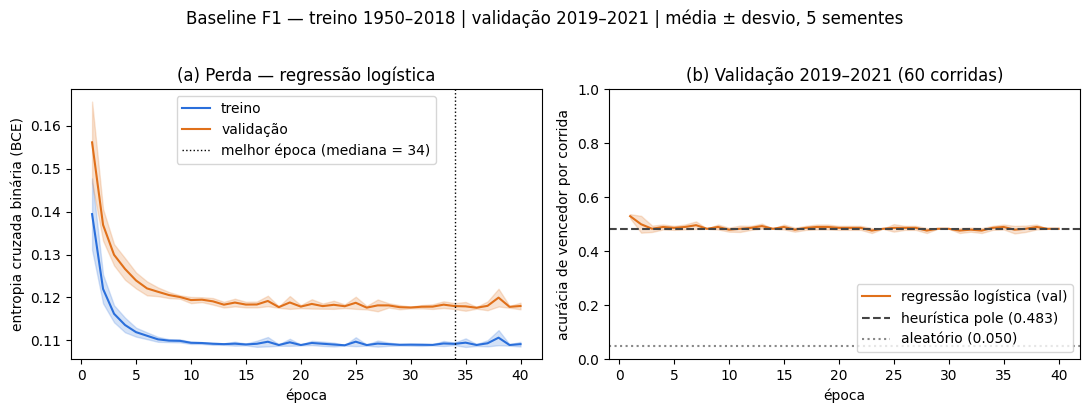
\includegraphics[width=\textwidth]{m2_baseline_colab.png}
  \caption{Baseline na valida\c{c}\~ao. (a) Entropia cruzada bin\'aria (BCE) de treino e valida\c{c}\~ao por \'epoca (m\'edia $\pm$ desvio de 5 sementes). (b) Acur\'acia de vencedor por corrida na valida\c{c}\~ao (2019--2021), contra a heur\'istica da pole e o palpite aleat\'orio.}
  \label{fig:baseline}
\end{figure}

\noindent Usamos o dataset p\'ublico do Kaggle \textit{Formula 1 World Championship (1950--2024)} (rohanrao), com divis\~ao estritamente temporal: treino 1950--2018 (24\,200 linhas, 997 corridas), valida\c{c}\~ao 2019--2021 (1\,200 linhas, 60 corridas); o teste (2022--2024) n\~ao foi tocado. A m\'etrica \'e a acur\'acia de vencedor por corrida (\textit{top-1}: em cada corrida o modelo escolhe um piloto e acerta se ele venceu), pois cerca de 96\,\% das linhas s\~ao ``n\~ao vence''. O \textit{baseline} \'e duplo e usa apenas informa\c{c}\~ao pr\'e-corrida: (i)~a heur\'istica ``a pole vence'', que obt\'em 0,483 na valida\c{c}\~ao, e (ii)~uma regress\~ao log\'istica (um neur\^onio sigmoide em PyTorch, Adam, 40 \'epocas, \textit{checkpoint} na melhor BCE de valida\c{c}\~ao) sobre a posi\c{c}\~ao de largada e a fra\c{c}\~ao de pontos da equipe no campeonato antes da prova, que obt\'em \textbf{0,490 $\pm$ 0,009} (m\'edia $\pm$ desvio de 5 sementes; BCE de valida\c{c}\~ao 0,1171 $\pm$ 0,0001), contra 0,050 de um palpite aleat\'orio. A regress\~ao log\'istica praticamente empata com a pole ($\Delta = +0{,}007$, dentro da dispers\~ao); como a valida\c{c}\~ao tem apenas 60 corridas, o erro-padr\~ao da acur\'acia \'e de cerca de 6,5 p.p., de modo que diferen\c{c}as menores que isso n\~ao s\~ao conclusivas. O tempo de execu\c{c}\~ao (dados, pr\'e-processamento e treino de 5 sementes) foi de \textbf{39,0\,s} no Google Colab (CPU, Python 3.13, PyTorch 2.14.1; dados 1,4\,s e treino das 5 sementes 25,0\,s). Este \'e o ponto de compara\c{c}\~ao que o MLP/XGBoost dever\'a superar em pelo menos 5\,\% (crit\'erio de empate do M1) no M3.

\medskip
\noindent\textbf{C\'odigo (Google Colab):} \href{https://colab.research.google.com/github/BalieroGu/jean-f1/blob/main/T2_M2_baseline.ipynb}{abrir o notebook no Colab}\\
\textbf{Reposit\'orio:} \url{https://github.com/BalieroGu/jean-f1}

\end{document}
